% !TeX root = 00General.tex
\thispagestyle{standard}
\pagestyle{standard}
\chapter{Network Reconnaissance}

\section{Network Ping Sweep}

In this part information about hosts in a connected network is gathered.
With the help of the Kali VM a \texttt{nmap} Ping Sweep command is executed to gather information of the connected devices within the network of the given IP.\\
\texttt{nmap -sP 172.16.1.*}

The information gathered are the IP address of the connected device and his MAC address.

\begin{figure}[H]
	\centering
	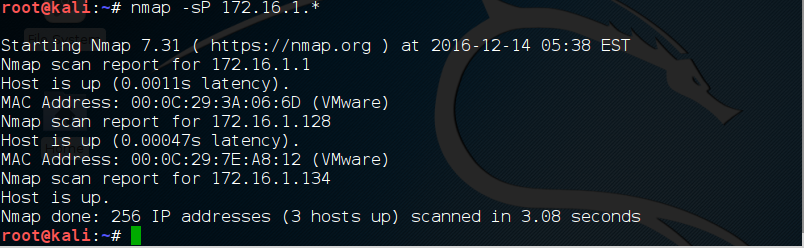
\includegraphics[width=0.9\textwidth]{img/2_1_Network_Ping_Sweep_Kali.PNG}
	\caption{Network Ping Sweep with Kali VM}
	\label{img:network ping sweep}
\end{figure}

After the switch to the Ubuntu VM we can analyze the Wireshark trace we started in first place. The trace shows that the \texttt{nmap} Ping Sweep command executes an \ac{ARP}-request on every host on the given IP network range. If a host is available he answers with his MAC address.

\textit{Advanced:}\\
If a system detects a certain amount of new \ac{ARP}-requests on every host system in a network then this could be a sign for an intrution. Since \ac{ARP} is a stateless protocol, hosts in the network can be compromised by spoofing with falsified IP-MAC pairs.

\section{OS Detection}

Informations about a specific host in the network are gathered. With the help of the Kali VM an OS detection command is executed.\\
\texttt{nmap -O -v 172.16.1.X}
\newpage
The gathered informations are:
\begin{itemize}  
\item Open ports
\item MAC address
\item Device type
\item The running operation system 
\item The network distance to the host (in hops)
\item TCP Sequence Prediction
\end{itemize}
With these information further steps can be planned and executed to compromise this specific host system.

\begin{figure}[H]
	\centering
	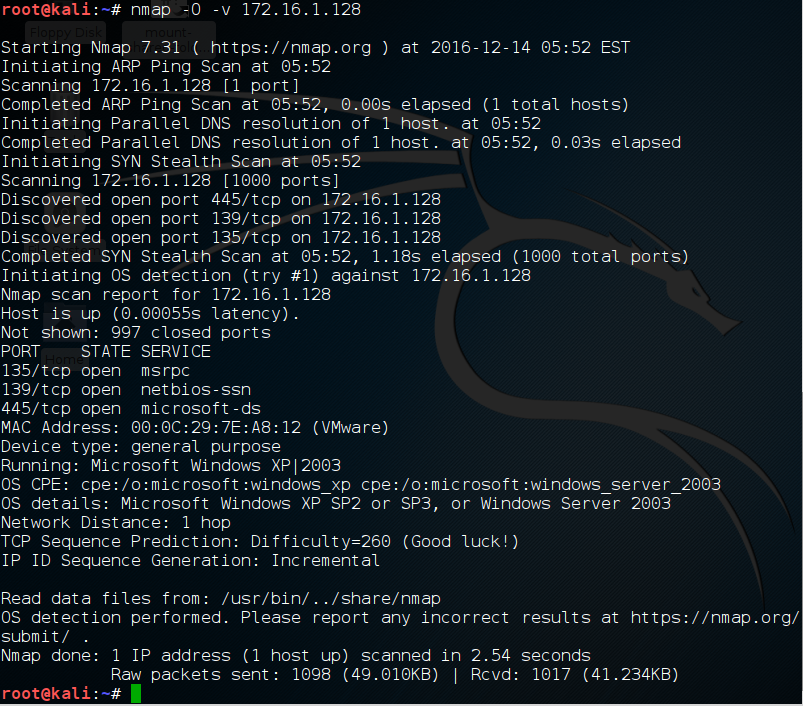
\includegraphics[width=0.9\textwidth]{img/2_2_OS_Detection_Kali.PNG}
	\caption{OS detection nmap command with Kali VM}
	\label{img:os detection kali}
\end{figure}

\section{Email Sniffing}

In this part Wireshark is used to listen to packets of the \ac{POP3} protocol. After receiving the authentication packets from the mail server a few \ac{POP3} packages can be found. One of the packets contains a character sequence which is base64-encoded (e.g. \texttt{"AHJla3RvcgByZWt0b3I"}). This sequence can then be decoded with an external decoder to the username and password of the client which tried to authenticate on the mail server (in this example it is \texttt{"rektor rektor"}).

After sending an receiving an email from the mail server an \ac{SMTP} packet can be found where the sender, receives, subject and the email text is shown in plaintext. When the attack is performed on the Kali VM it shows the same results (base64-decoded authentication and plaintext \ac{SMTP} packet).

\textit{Advanced:}\\
To let this attack be successful an non secured transport protocol need to be used and the used \ac{SMTP} needs to be in plain-text.
One counter-measure is the use of \ac{SSL} for \ac{SMTP} connections. This raises another problem. By default, all \ac{SMTP} servers use port 25. But if you use \ac{SSL} on port 25, non-\ac{SSL} will not be able to connect through that port. And if you use a non-standard port number, other servers will not be able to find your server.
Another counter-measure is the use of \ac{TLS} for an \ac{SMTP} connection. Each end of the connection can choose to authenticate the other, or the \ac{TLS} connection can be used purely for privacy. (http://windowsitpro.com/exchange-server/securing-smtp-email-traffic)

\chapter{Active Attacks}

\section{ARP Poisoning}

With the \ac{ARP} poisoning attack a host system should be compromised by sending out a wrong \ac{IP} and \ac{MAC} address assignment to the host. When the compromised host then wants to authenticate on the mail server he actually sends the username and password of his email account to the wrong \ac{IP} address.

\begin{figure}[H]
	\centering
	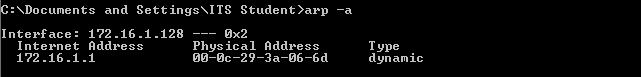
\includegraphics[width=0.9\textwidth]{img/3_1_Arp-a_Windows.PNG}
	\caption{arp -a before the ARP poisoning}
	\label{img:arp -a before}
\end{figure}

\begin{figure}[H]
	\centering
	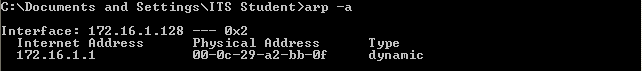
\includegraphics[width=0.9\textwidth]{img/3_1_arp-a_Windows_nach_poisoning.PNG}
	\caption{arp -a after the ARP poisoning}
	\label{img:arp -a after}
\end{figure}

\autoref{img:arp -a after} shows that a wrong \ac{MAC} address is now in the \ac{ARP} table.
Before ending the ettercap attack, ettercap sends out a new \ac{ARP} request with the correct \ac{IP} and \ac{MAC} address assignment to the host.

\textit{Advanced:}\\
\ac{ARP} spoofing is a so called Man In the Middle Attack. Mallory is between the communication of host A and B. To keep the attack alive he constantly needs to send wrong \ac{ARP} requests to both host A and B. If Mallory would not do this a new \ac{ARP} lookup would happen after a certain amount of time and this would replace the \ac{ARP} entry of Mallory.

\section{DHCP Spoofing}

During the attack the attacker listens on \ac{DHCP} request. Since the request is a broadcast everyone in the LAN will receive it. Normaly the real \ac{DHCP} server will reply to the request but since the attacker host, which simulates a \ac{DHCP} server is closer to the host that sent out the request, the host will receive the wrong \ac{DHCP} answer earlier. The host then stores the attacker host IP as default-gateway and all the communication passes the attacker.

A possible counter-measure against \ac{DHCP} spoofing is \ac{DHCP} snooping. This feature implement2 two different types of ports in a switched environment, trusted and untrusted ports. The first have no restrictions on \ac{DHCP} messages. If a unstrusted port then receives an incoming \ac{DHCP} packet it will be blocked.

\section{SSL Capturing}

With the use of \ac{ARP} poisoning a compromised communication from a host A to any kind of \ac{IP} address is established. If host A now wants to access a \ac{HTTPS} website, a certification notification occurs. If host A confirms this untrusted certification then the attacker has the private key which is used to decrypt the encrypt packets from the \ac{HTTPS} website. He then can find possible passwords.
This can be avoided by accepting only trusted certifications.

\chapter{Metasploit}

\section{Brute-Force Attacks}

Using the \texttt{"mysql\_login"} scanner-tool from the metasploit framework executed a brute-force attack onto the host \texttt{"10.1.1.10"} which is the metasploitable linux distribution. First the list of all usernames and passwords have to be set wit a few commands. Also the \ac{IP} of the host has to be set. Afterwards the attack can be started by using the \texttt{run} command. The attack showed that the username \texttt{root} can be accessed with the password \texttt{root}.

\section{Tomcat}

Using the \texttt{"tomcat\_mgr\_login"} scanner-tool from the metasploit framework executed a brute-force attack onto the host \texttt{"10.1.1.10"} which is the metasploitable linux distribution. First the list of all usernames and passwords have to be set wit a few commands. Also the \ac{IP} of the host has to be set. Afterwards the attack can be started by using the \texttt{run} command. Running an OS detection scan on the host \ac{IP} showed an unknown port \texttt{8180}. This port was later used to be set in the scanner-tool via \texttt{"set RPORT 8180"}. The attack showed that the username \texttt{tomcat} can be accessed with the password \texttt{tomcat}. Since tomcat uses a web-interface for e.g. managing applications, the web-interface can be accessed with \texttt{"10.1.1.10:8180"}. Then the "Tomcat Web Application Manager" can be accessed with username and password.

\section{Summary}

Systems can easily be hacked with brute-force attacks. Since the computing power is rising longer passwords or other security mechanism are needed to be safe. One of those can be a limit of maximum number of tries in a certain amount of time. Another one can be captchas. An administrator of a webserver for example can implement such counter-measures to limit the brute-force attacks although such attacks are difficult to stop completely.

\chapter{Counter Measures}

At first the \texttt{"auth.log"} displays all the incorrect ssh-login attempts with the \ac{IP} of the host from which the login happened. After applying the firewall rule \texttt{"iptables -A INPUT -s 172.16.1.134 -p tcp -j DROP"} the brute-force output on the Kali VM showed that the connection timed out. When using \texttt{fail2ban} the \ac{IP} address of the host with too many failed login tries will be automatically addded to the iptable.